\section{Model analityczny}
Celem niniejszego rozdziału jest zdefiniowanie, jak wyglądać będzie architektura tworzonego systemu. Aby to osiągnąć, w~rozdziale załączone zostały diagramy wykonane zgodnie ze~standardem UML, które stanowią wizualną reprezentację architektury systemu oraz pozwalają na~łatwiejszą analizę stanu projektu.

\subsection{Diagram klas}
Przedstawiony poniżej diagram klas reprezentuje wszystkie wykorzystywane przez Zleceniodawcę elementy składające się na cały system. Diagram ten jest kluczowy przede wszystkim dla deweloperów oraz innych osób zajmujących się bezpośrednio wytwarzaniem oprogramowania, tym niemniej powinien zostać zatwierdzony także przez przedstawicieli Zleceniodawcy -- diagram klas jest bowiem punktem łączącym -- z~jednej strony wyobrażenie klienta o~podziale funkcjonalności, a~z~drugiej decyzje projektowe podjęte przez zespół zajmujący się implementacją.\\

\begin{figure}[H]
  \centering
  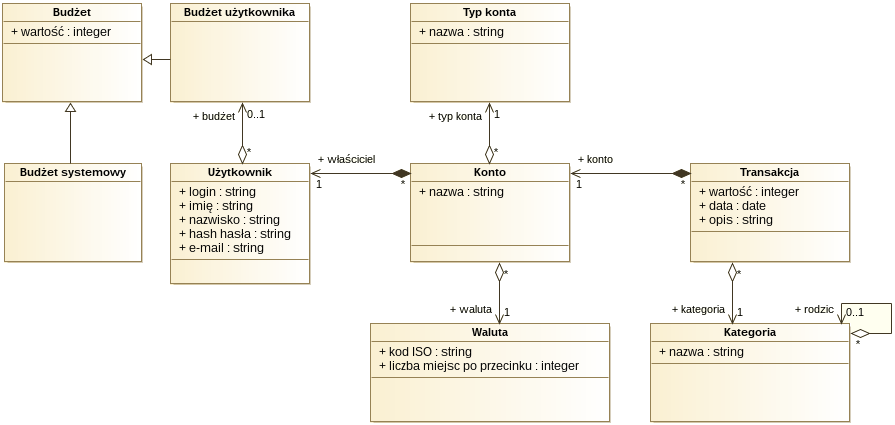
\includegraphics[width=\textwidth]{images/class-diagram.png}
  \caption{Diagram klas systemu.}
\end{figure}

Diagram klas obrazuje zależności (agregacje, kompozycje, relacje dziedziczenia) pomiędzy poszczególnymi klasami na~tyle szczegółowo, by~osoby nieposiadające wykształcenia informatycznego i~nieznające metod programowania obiektowego mogły zrozumieć zasadę podziału bez szczegółowych wyjaśnień. Wszystkie atrybuty czy operacje ważne z~punktu widzenia Zleceniodawcy, które mogą mieć wpływ na~ocenę projektu zostały umieszczone na~diagramie. Poniżej umieszczony został opis każdej z~klas.\\

\textbf{Użytkownik} reprezentuję osobę korzystającą z~aplikacji. Klasa ta~zawiera istotne informacje potrzebne głównie do~uwierzytelniania, takie jak login oraz hash hasła. Pozostałe pola to~na~przykład imię i~nazwisko, czy adres e-mail.\\

\textbf{Konto} jest klasą reprezentującą konto pieniężne (np. oszczędnościowe, osobiste, czy walutowe), które należy do~danego użytkownika. Klasa ta~posiada pola, takie jak nazwa, typ, waluta oraz bieżące saldo.\\

\textbf{Typ konta} jest klasą wydzieloną z~klasy Konto. Utworzenie tej klasy pozwoli na~ograniczenie wartości wprowadzanych w~polu typ konta.\\

\textbf{Waluta} jest kolejną klasą wydzieloną z~klasy Konto. Utworzenie tej klasy pozwoli na~ograniczenie wartości wprowadzanych w~polu waluta. Ponadto przechowuje ona liczbę miejsc po~przecinku, na~jakie zezwala dana waluta, a~więc pozwoli na~walidację wartości pieniężnych wprowadzanych przez użytkownika do~systemu.\\

\textbf{Transakcja} reprezentuje przepływ pieniędzy między kontami. Istnieją trzy typy transakcji -- przychody (pieniądze pochodzące z~konta poza systemem, które trafiają na~jedno z~kont użytkownika), koszty (pieniądze pochodzące z~jednego z~kont użytkownika, które trafiają na~konto poza systemem), lub przelew (pieniądze transferowane pomiędzy dwoma kontami, oba należące do tego samego użytkownika). Klasa ta~zawiera także inne pola, takie jak data, opis (opcjonalnie), czy wartość pieniężna.\\

\textbf{Kategoria} reprezentuje etykiety, które mogą być przypisane do~transakcji. Podobnie jak klasy Waluta oraz Typ konta, jest to~klasa wydzielona z~innej klasy, w~tym przypadku z~Transakcji. Zawiera tylko pole przechowujące nazwę. Kategorie tworzą strukturę drzewa -- jest to~dozwolone poprzez rekurencyjną relację jeden-do-wielu.\\

\textbf{Budżet} jest klasą abstrakcyjną reprezentującą budżet, czyli ograniczenie nakładane na~użytkownika lub cały system. Zawiera ona~tylko jedno pole -- wartość ograniczenia. Istnieją dwie klasy dziedziczące po~klasie Budżet: Budżet użytkownika oraz Budżet systemowy, odpowiednio reprezentują one ograniczenia nałożone na~konkretnego użytkownika, lub cały system.\\
